\documentclass[11pt,a4paper]{report}

% ============================================================================
% PACKAGES
% ============================================================================

% Encoding and fonts
\usepackage[utf8]{inputenc}
\usepackage[T1]{fontenc}
\usepackage{lmodern}

% Page layout
\usepackage[margin=2.5cm]{geometry}
\usepackage{parskip}

% Colors
\usepackage[dvipsnames,table]{xcolor}
\definecolor{codeblue}{RGB}{37,99,235}
\definecolor{codegray}{RGB}{107,114,128}
\definecolor{codegreen}{RGB}{34,197,94}
\definecolor{codered}{RGB}{239,68,68}
\definecolor{codebg}{RGB}{249,250,251}
\definecolor{linkblue}{RGB}{37,99,235}

% Hyperlinks
\usepackage[colorlinks=true,linkcolor=linkblue,urlcolor=linkblue,citecolor=linkblue]{hyperref}

% Code listings
\usepackage{listings}
\lstdefinestyle{yaml}{
    backgroundcolor=\color{codebg},
    basicstyle=\ttfamily\small,
    breaklines=true,
    frame=single,
    framesep=5pt,
    rulecolor=\color{gray!30},
    commentstyle=\color{codegray},
    keywordstyle=\color{codeblue},
    stringstyle=\color{codegreen},
    numbers=none,
    showstringspaces=false,
    tabsize=2,
}

\lstdefinestyle{bash}{
    backgroundcolor=\color{codebg},
    basicstyle=\ttfamily\small,
    breaklines=true,
    frame=single,
    framesep=5pt,
    rulecolor=\color{gray!30},
    keywordstyle=\color{codeblue},
    numbers=none,
    showstringspaces=false,
}

\lstset{style=yaml}

% Tables
\usepackage{booktabs}
\usepackage{longtable}
\usepackage{array}
\usepackage{multirow}

% Graphics and diagrams
\usepackage{tikz}
\usetikzlibrary{arrows.meta,positioning,shapes.geometric,calc,fit,backgrounds}

% Lists
\usepackage{enumitem}

% Math
\usepackage{amsmath}

% Captions
\usepackage{caption}

% Header and footer
\usepackage{fancyhdr}
\pagestyle{fancy}
\fancyhf{}
\fancyhead[L]{\leftmark}
\fancyhead[R]{Prompt Evaluation Pipeline}
\fancyfoot[C]{\thepage}
\renewcommand{\headrulewidth}{0.4pt}

% Title formatting
\usepackage{titlesec}
\titleformat{\chapter}[display]
  {\normalfont\huge\bfseries}{\chaptertitlename\ \thechapter}{20pt}{\Huge}

% ============================================================================
% DOCUMENT INFO
% ============================================================================

\title{
    \vspace{-2cm}
    \textbf{Prompt Evaluation Pipeline}\\
    \vspace{0.5cm}
    \large Complete Documentation\\
    \vspace{0.3cm}
    \normalsize Version 0.1.0
}

\author{
    A Declarative YAML-Based Framework\\
    for Testing and Comparing LLM Prompts
}

\date{\today}

% ============================================================================
% DOCUMENT
% ============================================================================

\begin{document}

\maketitle

\tableofcontents

\newpage

% ============================================================================
% CHAPTER 1: INTRODUCTION
% ============================================================================

\chapter{Introduction}

\section{What is Prompt Engineering?}

\textbf{Prompt engineering} is the practice of designing, refining, and optimizing the instructions (prompts) given to Large Language Models (LLMs) to achieve desired outputs. It involves:

\begin{itemize}
    \item \textbf{Crafting clear instructions}: Writing precise directions that guide the model's behavior
    \item \textbf{Providing context}: Including relevant background information to improve response quality
    \item \textbf{Setting constraints}: Defining boundaries for format, length, tone, and content
    \item \textbf{Using examples}: Demonstrating expected input-output patterns (few-shot learning)
    \item \textbf{Iterative refinement}: Testing and improving prompts based on observed results
\end{itemize}

Prompt engineering is crucial because the same model can produce vastly different results depending on how instructions are framed. A well-engineered prompt can be the difference between a helpful, accurate response and a vague or incorrect one.

\subsection{Example of Prompt Engineering Evolution}

\begin{lstlisting}[style=yaml,title={Version 1 (Basic)}]
"Answer the user's question."
\end{lstlisting}

\begin{lstlisting}[style=yaml,title={Version 2 (With context)}]
"You are a helpful customer support assistant. Answer the user's
question clearly and concisely."
\end{lstlisting}

\begin{lstlisting}[style=yaml,title={Version 3 (With constraints)}]
"You are a helpful customer support assistant for TechCorp. Answer
the user's question in 2-3 sentences. If you don't know the answer,
say 'I'll need to check with our team.' Never make up information."
\end{lstlisting}

\section{What is Prompt Evaluation?}

\textbf{Prompt evaluation} is the systematic process of testing prompts against predefined criteria to measure their quality, consistency, and effectiveness. It answers the question: \textit{``How well does this prompt perform?''}

Prompt evaluation involves:

\begin{itemize}
    \item \textbf{Defining test cases}: Creating representative inputs with expected outcomes
    \item \textbf{Running evaluations}: Executing prompts against test cases and capturing outputs
    \item \textbf{Measuring quality}: Applying metrics to quantify how well outputs meet expectations
    \item \textbf{Comparing versions}: Testing multiple prompt variants to identify the best performer
    \item \textbf{Tracking regression}: Ensuring prompt changes don't degrade quality over time
\end{itemize}

\subsection{Why is Prompt Evaluation Important?}

\begin{table}[h]
\centering
\begin{tabular}{@{}p{5cm}p{8cm}@{}}
\toprule
\textbf{Problem} & \textbf{Solution through Evaluation} \\
\midrule
Inconsistent outputs & Measure consistency across multiple test cases \\
Quality degradation after changes & Run regression tests before deployment \\
Difficulty choosing between prompt versions & Compare metrics side-by-side \\
No objective quality measurement & Apply quantifiable metrics (accuracy, relevance) \\
Manual testing is time-consuming & Automate with declarative test configurations \\
\bottomrule
\end{tabular}
\caption{Problems solved by prompt evaluation}
\end{table}

\section{Why Use This Framework?}

The \textbf{Prompt Evaluation Pipeline} provides:

\begin{itemize}
    \item \textbf{Declarative configuration}: Define evaluations in YAML without writing code
    \item \textbf{Multiple metrics}: Built-in support for exact match, substring search, length validation, regex patterns, and LLM-based judging
    \item \textbf{Batch evaluation}: Run multiple test cases automatically
    \item \textbf{Prompt comparison}: Evaluate multiple prompt versions side-by-side
    \item \textbf{Multiple export formats}: Generate reports in JSON, CSV, Markdown, and HTML
    \item \textbf{Prompt caching}: Optimize API costs with Anthropic's prompt caching feature
    \item \textbf{Extensible design}: Easy to add custom metrics and exporters
\end{itemize}

% ============================================================================
% CHAPTER 2: QUICK START
% ============================================================================

\chapter{Quick Start}

Get started in 5 minutes:

\section{Step 1: Install the Package}

\begin{lstlisting}[style=bash]
pip install -e .
\end{lstlisting}

\section{Step 2: Set Your API Key}

\begin{lstlisting}[style=bash]
export ANTHROPIC_API_KEY=your_key_here
\end{lstlisting}

\section{Step 3: Create a Prompt File}

Create the file \texttt{prompts/qa\_assistant.yaml}:

\begin{lstlisting}[style=yaml]
name: qa_assistant_v1
version: "1.0"
description: "A helpful Q&A assistant"
system: |
  You are a helpful Q&A assistant. Answer questions accurately
  and concisely. If you don't know the answer, say "I don't know."
template: |
  Question: {question}
\end{lstlisting}

\section{Step 4: Create an Evaluation Config}

Create the file \texttt{configs/eval\_qa.yaml}:

\begin{lstlisting}[style=yaml]
model: claude-sonnet-4-20250514
max_tokens: 256
temperature: 0.0
evaluation_threshold: 0.8

prompts:
  - prompts/qa_assistant.yaml

test_cases:
  - name: capital_france
    inputs:
      question: "What is the capital of France?"
    expected_contains:
      - "Paris"

  - name: unknown_question
    inputs:
      question: "What color is the invisible dragon?"
    expected_contains:
      - "don't know"

metrics:
  - type: contains
    case_sensitive: false
\end{lstlisting}

\section{Step 5: Run the Evaluation}

\begin{lstlisting}[style=bash]
prompt-eval run configs/eval_qa.yaml
\end{lstlisting}

\section{Step 6: View Results}

Results are saved in \texttt{results/qa/<timestamp>/} with JSON, CSV, Markdown, and HTML reports.

% ============================================================================
% CHAPTER 3: INSTALLATION
% ============================================================================

\chapter{Installation}

\section{Requirements}

\begin{itemize}
    \item Python 3.10 or higher
    \item An Anthropic API key
\end{itemize}

\section{Installation Steps}

\subsection{Option A: Install from Source (Recommended)}

\begin{lstlisting}[style=bash]
# Clone the repository
git clone https://github.com/your-org/prompt-eval-pipeline.git
cd prompt-eval-pipeline

# Create a virtual environment
python -m venv venv
source venv/bin/activate  # On Windows: venv\Scripts\activate

# Install in editable mode
pip install -e .

# Install development dependencies (optional)
pip install -e ".[dev]"
\end{lstlisting}

\subsection{Option B: Install Dependencies Manually}

\begin{lstlisting}[style=bash]
pip install anthropic>=0.40.0 pydantic>=2.0.0 pyyaml>=6.0 \
    rich>=13.0.0 pandas>=2.0.0 jinja2>=3.0.0 click>=8.0.0 \
    python-dotenv>=1.0.0 pypdf>=5.0.0
\end{lstlisting}

\section{Configuration}

\subsection{Setting the API Key}

\textbf{Option 1:} Environment variable
\begin{lstlisting}[style=bash]
export ANTHROPIC_API_KEY=sk-ant-...
\end{lstlisting}

\textbf{Option 2:} Create a \texttt{.env} file in the project root
\begin{lstlisting}
ANTHROPIC_API_KEY=sk-ant-...
\end{lstlisting}

\subsection{Verify Installation}

\begin{lstlisting}[style=bash]
prompt-eval --version
# Output: prompt-eval, version 0.1.0
\end{lstlisting}

% ============================================================================
% CHAPTER 4: ARCHITECTURE
% ============================================================================

\chapter{Architecture Overview}

The framework follows a modular architecture with clear separation of concerns.

\section{Architecture Diagram}

\begin{figure}[h]
\centering
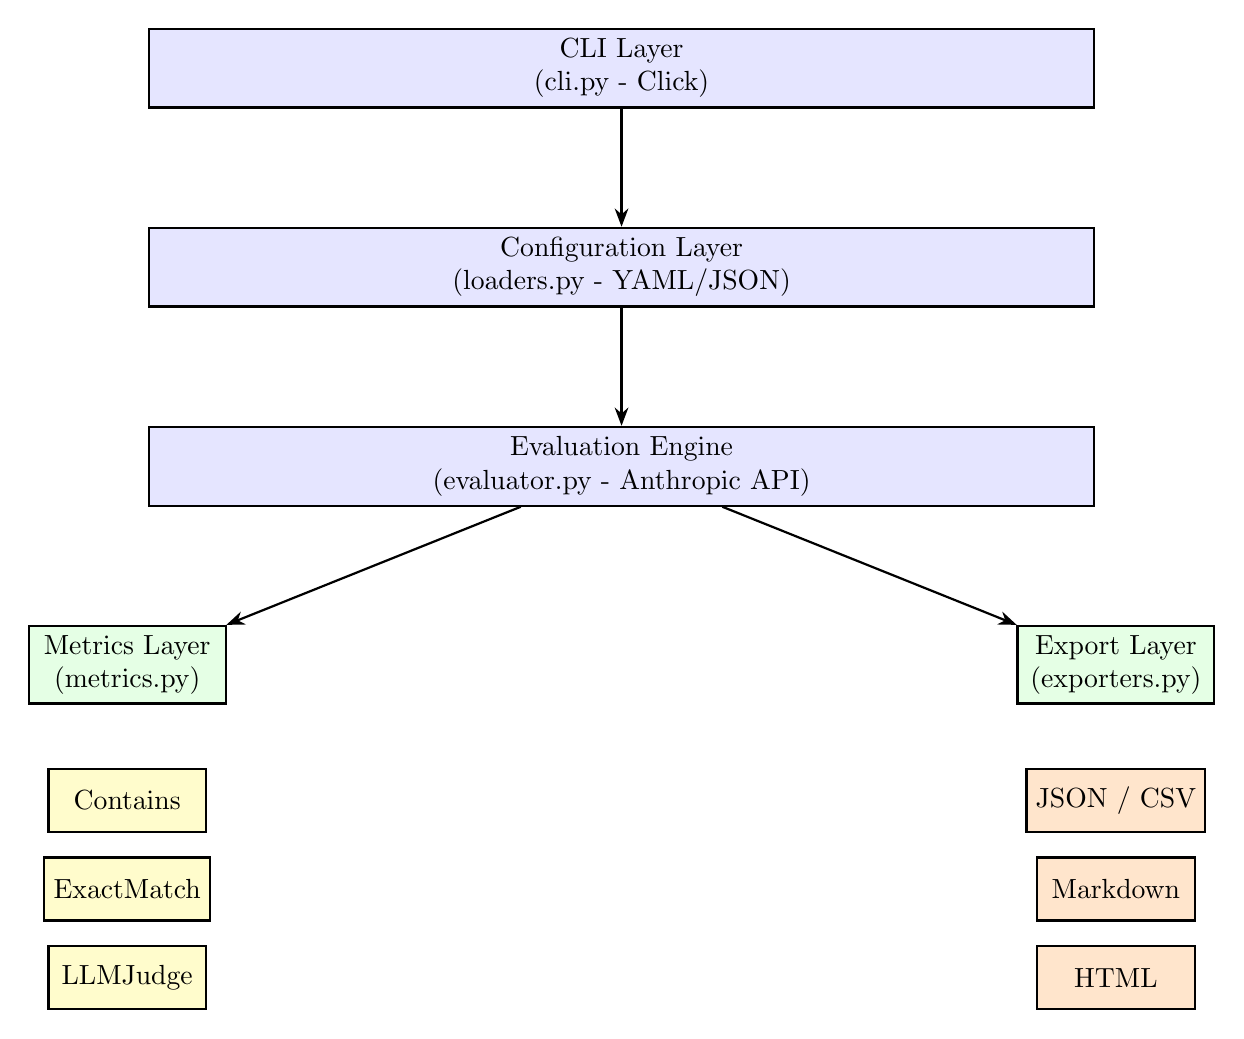
\begin{tikzpicture}[
    box/.style={rectangle, draw=black, thick, minimum height=1cm, minimum width=4cm, align=center, fill=blue!10},
    smallbox/.style={rectangle, draw=black, thick, minimum height=0.8cm, minimum width=2.5cm, align=center, fill=green!10},
    arrow/.style={-{Stealth}, thick},
    node distance=1.5cm
]

% CLI Layer
\node[box, minimum width=12cm] (cli) {CLI Layer\\(cli.py - Click)};

% Config Layer
\node[box, minimum width=12cm, below=of cli] (config) {Configuration Layer\\(loaders.py - YAML/JSON)};

% Evaluation Engine
\node[box, minimum width=12cm, below=of config] (eval) {Evaluation Engine\\(evaluator.py - Anthropic API)};

% Bottom layers
\node[smallbox, below left=1.5cm and -1cm of eval] (metrics) {Metrics Layer\\(metrics.py)};
\node[smallbox, below right=1.5cm and -1cm of eval] (export) {Export Layer\\(exporters.py)};

% Metric types
\node[smallbox, below=0.8cm of metrics, minimum width=2cm, fill=yellow!20] (m1) {Contains};
\node[smallbox, below=0.3cm of m1, minimum width=2cm, fill=yellow!20] (m2) {ExactMatch};
\node[smallbox, below=0.3cm of m2, minimum width=2cm, fill=yellow!20] (m3) {LLMJudge};

% Export types
\node[smallbox, below=0.8cm of export, minimum width=2cm, fill=orange!20] (e1) {JSON / CSV};
\node[smallbox, below=0.3cm of e1, minimum width=2cm, fill=orange!20] (e2) {Markdown};
\node[smallbox, below=0.3cm of e2, minimum width=2cm, fill=orange!20] (e3) {HTML};

% Arrows
\draw[arrow] (cli) -- (config);
\draw[arrow] (config) -- (eval);
\draw[arrow] (eval) -- (metrics);
\draw[arrow] (eval) -- (export);

\end{tikzpicture}
\caption{Prompt Evaluation Pipeline Architecture}
\end{figure}

\section{Component Responsibilities}

\begin{table}[h]
\centering
\begin{tabular}{@{}llp{7cm}@{}}
\toprule
\textbf{Component} & \textbf{File} & \textbf{Responsibility} \\
\midrule
CLI & cli.py & Command-line interface, orchestration \\
Loaders & loaders.py & Parse YAML/JSON configurations \\
Models & models.py & Data structures (Prompt, TestCase, EvalResult) \\
Evaluator & evaluator.py & Execute prompts, call Anthropic API \\
Metrics & metrics.py & Score outputs against expectations \\
Exporters & exporters.py & Generate reports in multiple formats \\
\bottomrule
\end{tabular}
\caption{Component responsibilities}
\end{table}

% ============================================================================
% CHAPTER 5: CLI REFERENCE
% ============================================================================

\chapter{CLI Reference}

\section{Main Command}

\begin{lstlisting}[style=bash]
prompt-eval [OPTIONS] COMMAND [ARGS]
\end{lstlisting}

\textbf{Global Options:}
\begin{itemize}
    \item \texttt{--version}: Show version and exit
    \item \texttt{--help}: Show help message and exit
\end{itemize}

\section{Run Command}

Execute an evaluation from a configuration file.

\begin{lstlisting}[style=bash]
prompt-eval run [OPTIONS] CONFIG_FILE
\end{lstlisting}

\textbf{Arguments:}
\begin{itemize}
    \item \texttt{CONFIG\_FILE}: Path to the evaluation configuration file (YAML or JSON)
\end{itemize}

\textbf{Options:}

\begin{table}[h]
\centering
\begin{tabular}{@{}llp{5cm}l@{}}
\toprule
\textbf{Option} & \textbf{Short} & \textbf{Description} & \textbf{Default} \\
\midrule
\texttt{--output} & \texttt{-o} & Output directory for results & Auto-generated \\
\texttt{--format} & \texttt{-f} & Output format & \texttt{all} \\
\texttt{--model} & \texttt{-m} & Override model from config & Config value \\
\texttt{--verbose} & \texttt{-v} & Enable verbose output & True \\
\texttt{--quiet} & \texttt{-q} & Disable verbose output & False \\
\bottomrule
\end{tabular}
\caption{Run command options}
\end{table}

\textbf{Format options:} \texttt{json}, \texttt{csv}, \texttt{markdown}, \texttt{html}, \texttt{all}

\section{Examples}

\begin{lstlisting}[style=bash]
# Basic run
prompt-eval run configs/eval_qa.yaml

# Specify output directory
prompt-eval run configs/eval_qa.yaml -o results/experiment1

# Only generate JSON output
prompt-eval run configs/eval_qa.yaml -f json

# Override model
prompt-eval run configs/eval_qa.yaml -m claude-opus-4-5-20251101

# Quiet mode (minimal output)
prompt-eval run configs/eval_qa.yaml -q
\end{lstlisting}

% ============================================================================
% CHAPTER 6: CONFIGURATION REFERENCE
% ============================================================================

\chapter{Configuration Reference}

\section{Evaluation Configuration}

The main configuration file defines the evaluation parameters.

\begin{lstlisting}[style=yaml,title={configs/eval\_<name>.yaml}]
# Model Configuration
model: claude-sonnet-4-20250514    # Required: Anthropic model ID
max_tokens: 1024                    # Optional: Max response tokens
temperature: 0.0                    # Optional: Sampling temperature
evaluation_threshold: 0.8           # Required: Pass/fail threshold

# Prompts to evaluate
prompts:
  - prompts/assistant_v1.yaml
  - prompts/assistant_v2.yaml

# Test cases
test_cases:
  - name: test_1
    inputs:
      question: "What is 2+2?"
    expected_contains:
      - "4"

# Metrics configuration
metrics:
  - type: contains
    case_sensitive: false
\end{lstlisting}

\section{Prompt Configuration}

Prompts define the instructions sent to the LLM.

\begin{lstlisting}[style=yaml,title={prompts/<name>.yaml}]
# Basic Information
name: qa_assistant_v1              # Required: Unique identifier
version: "1.0"                      # Optional: Version string
description: "Q&A assistant"        # Optional: Description

# Prompt Content
system: |                           # Optional: System prompt
  You are a helpful assistant.

template: |                         # Required: User prompt template
  Question: {question}

# Advanced Prompt Engineering
rules:                              # Optional: Behavioral rules
  - Always be polite
  - Never make up information

skills:                             # Optional: Skills/capabilities
  - Answering factual questions
  - Explaining complex topics

thinking_process: |                 # Optional: Chain-of-thought
  1. Understand the question
  2. Formulate a clear answer

examples:                           # Optional: Few-shot examples
  - input: "What is the sun?"
    output: "The sun is a star."

# File Caching
cached_files:                       # Optional: Files to cache
  - reference/knowledge_base.md
\end{lstlisting}

\section{Configuration Parameters Summary}

\begin{table}[h]
\centering
\begin{tabular}{@{}lllp{5cm}@{}}
\toprule
\textbf{Parameter} & \textbf{Required} & \textbf{Type} & \textbf{Description} \\
\midrule
\texttt{model} & Yes & string & Anthropic model ID \\
\texttt{max\_tokens} & No & int & Max response tokens (default: 1024) \\
\texttt{temperature} & No & float & Sampling temperature (default: 0.0) \\
\texttt{evaluation\_threshold} & Yes & float & Pass/fail threshold 0.0--1.0 \\
\texttt{prompts} & Yes & list & Prompt file paths or inline defs \\
\texttt{test\_cases} & Yes & list & Test case definitions \\
\texttt{metrics} & No & list & Metric configurations \\
\bottomrule
\end{tabular}
\caption{Configuration parameters}
\end{table}

% ============================================================================
% CHAPTER 7: METRICS REFERENCE
% ============================================================================

\chapter{Metrics Reference}

Metrics measure how well the LLM output matches expectations.

\section{Contains Metric}

Checks if the output contains required substrings and excludes forbidden ones.

\begin{lstlisting}[style=yaml]
metrics:
  - type: contains
    case_sensitive: false    # Optional (default: false)
\end{lstlisting}

\textbf{Scoring:}
\begin{equation}
\text{Score} = \min\left(\frac{\text{matched required}}{\text{total required}}, 1 - \frac{\text{violations}}{\text{total forbidden}}\right)
\end{equation}

\section{Exact Match Metric}

Checks if the output exactly matches the expected value.

\begin{lstlisting}[style=yaml]
metrics:
  - type: exact_match
    case_sensitive: false    # Optional (default: false)
    strip: true              # Optional (default: true)
\end{lstlisting}

\textbf{Scoring:} Binary (1.0 if match, 0.0 otherwise)

\section{Response Length Metric}

Validates the response length in characters or words.

\begin{lstlisting}[style=yaml]
metrics:
  - type: response_length
    min_chars: 100           # Optional
    max_chars: 500           # Optional
    min_words: 20            # Optional
    max_words: 100           # Optional
\end{lstlisting}

\textbf{Scoring:} Binary (1.0 if within bounds, 0.0 otherwise)

\section{Regex Match Metric}

Checks if the output matches a regular expression pattern.

\begin{lstlisting}[style=yaml]
metrics:
  - type: regex_match
    pattern: "\\d{4}-\\d{2}-\\d{2}"    # Date pattern
\end{lstlisting}

\section{LLM Judge Metric}

Uses another LLM to evaluate the quality of the output.

\begin{lstlisting}[style=yaml]
metrics:
  - type: llm_judge
    criteria: |
      Evaluate if the response is:
      1. Accurate and factual
      2. Clear and well-organized
    model: claude-sonnet-4-20250514
\end{lstlisting}

\section{Metrics Summary}

\begin{table}[h]
\centering
\begin{tabular}{@{}lp{5cm}l@{}}
\toprule
\textbf{Metric} & \textbf{Use Case} & \textbf{Scoring} \\
\midrule
\texttt{contains} & Check for required/forbidden content & Ratio of matches \\
\texttt{exact\_match} & Precise output matching & Binary (0 or 1) \\
\texttt{response\_length} & Enforce length constraints & Binary (0 or 1) \\
\texttt{regex\_match} & Pattern validation & Binary (0 or 1) \\
\texttt{llm\_judge} & Subjective quality assessment & Continuous (0--1) \\
\texttt{composite} & Combined evaluation & Weighted average \\
\bottomrule
\end{tabular}
\caption{Metrics summary}
\end{table}

% ============================================================================
% CHAPTER 8: TUTORIAL
% ============================================================================

\chapter{Tutorial: Building a Q\&A Chatbot Evaluation}

This tutorial walks through creating a complete evaluation pipeline for a Q\&A chatbot assistant.

\section{Scenario}

You're building a general-purpose Q\&A chatbot that should:
\begin{itemize}
    \item Answer factual questions accurately
    \item Admit when it doesn't know something
    \item Provide concise but complete answers
    \item Avoid making up information
\end{itemize}

\section{Step 1: Create the Project Structure}

\begin{lstlisting}
my-qa-chatbot/
    prompts/
        qa_v1.yaml
        qa_v2.yaml
    configs/
        eval_qa.yaml
    results/
\end{lstlisting}

\section{Step 2: Define Prompt Version 1}

\begin{lstlisting}[style=yaml,title={prompts/qa\_v1.yaml}]
name: qa_chatbot_v1
version: "1.0"
description: "Basic Q&A chatbot - first iteration"

system: |
  You are a helpful Q&A assistant. Answer user questions accurately.

template: |
  User Question: {question}
\end{lstlisting}

\section{Step 3: Define Prompt Version 2 (Improved)}

\begin{lstlisting}[style=yaml,title={prompts/qa\_v2.yaml}]
name: qa_chatbot_v2
version: "2.0"
description: "Improved Q&A chatbot with better instructions"

system: |
  You are a knowledgeable and helpful Q&A assistant.

rules:
  - Provide accurate, factual information
  - Keep answers concise (2-4 sentences for simple questions)
  - If you don't know, say "I don't have information about that"
  - Never make up facts or statistics

thinking_process: |
  1. Understand what the user is asking
  2. Determine if I have reliable information
  3. Formulate a clear response or admit ignorance

template: |
  Please answer the following question:
  {question}
\end{lstlisting}

\section{Step 4: Create Test Cases}

\begin{lstlisting}[style=yaml,title={configs/eval\_qa.yaml}]
model: claude-sonnet-4-20250514
max_tokens: 512
temperature: 0.0
evaluation_threshold: 0.8

prompts:
  - prompts/qa_v1.yaml
  - prompts/qa_v2.yaml

test_cases:
  # Factual questions
  - name: capital_france
    inputs:
      question: "What is the capital of France?"
    expected_contains:
      - "Paris"
    tags: [geography, factual]

  - name: water_formula
    inputs:
      question: "What is the chemical formula for water?"
    expected_contains:
      - "H2O"
    tags: [science, factual]

  # Unknown questions
  - name: unknown_personal
    inputs:
      question: "What did I have for breakfast yesterday?"
    expected_contains:
      - "don't"
    expected_not_contains:
      - "you had"
    tags: [unknown, boundary]

metrics:
  - type: contains
    case_sensitive: false
  - type: response_length
    min_words: 5
    max_words: 200
\end{lstlisting}

\section{Step 5: Run and Analyze}

\begin{lstlisting}[style=bash]
prompt-eval run configs/eval_qa.yaml
\end{lstlisting}

Results will show which prompt version performs better across all test cases.

% ============================================================================
% CHAPTER 9: SEQUENCE DIAGRAMS
% ============================================================================

\chapter{Sequence Diagrams}

\section{Single Prompt Evaluation Flow}

\begin{figure}[h]
\centering
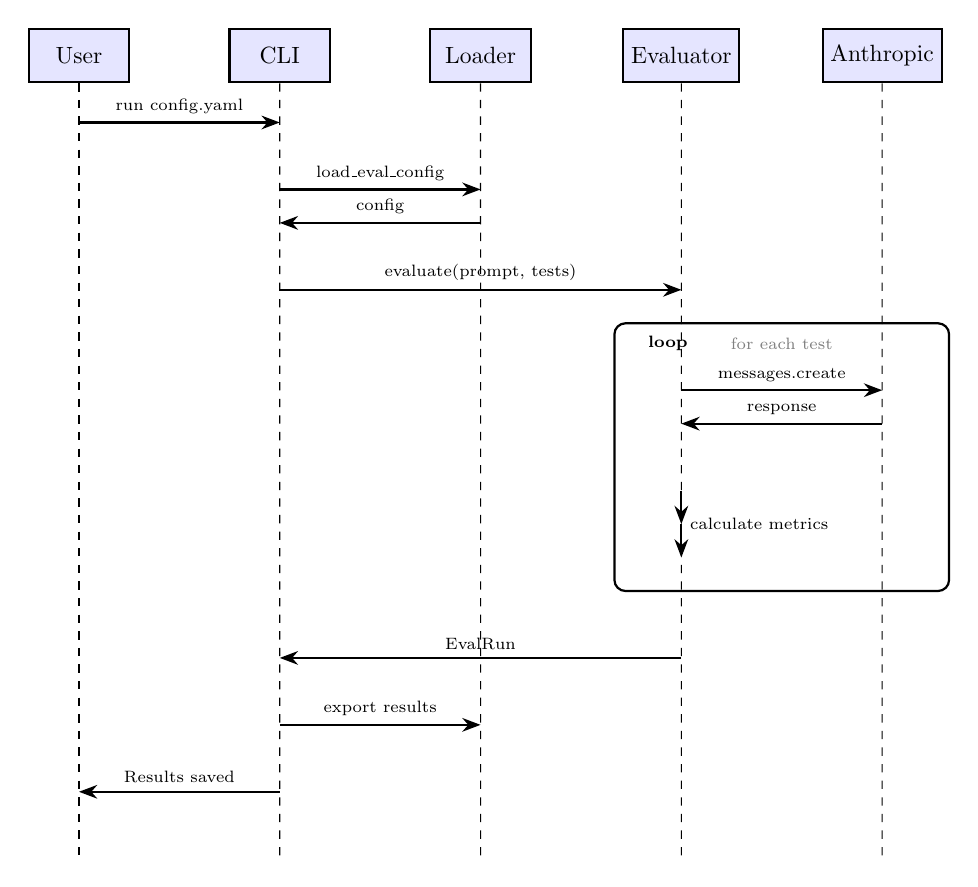
\begin{tikzpicture}[
    actor/.style={rectangle, draw=black, thick, minimum height=0.8cm, minimum width=1.5cm, fill=blue!10},
    arrow/.style={-{Stealth}, thick},
    note/.style={rectangle, draw=gray, dashed, fill=yellow!10, font=\small},
    scale=0.85, transform shape
]

% Actors
\node[actor] (user) at (0,0) {User};
\node[actor] (cli) at (3,0) {CLI};
\node[actor] (loader) at (6,0) {Loader};
\node[actor] (eval) at (9,0) {Evaluator};
\node[actor] (api) at (12,0) {Anthropic};

% Lifelines
\draw[dashed] (user) -- (0,-12);
\draw[dashed] (cli) -- (3,-12);
\draw[dashed] (loader) -- (6,-12);
\draw[dashed] (eval) -- (9,-12);
\draw[dashed] (api) -- (12,-12);

% Messages
\draw[arrow] (0,-1) -- node[above, font=\scriptsize] {run config.yaml} (3,-1);
\draw[arrow] (3,-2) -- node[above, font=\scriptsize] {load\_eval\_config} (6,-2);
\draw[arrow] (6,-2.5) -- node[above, font=\scriptsize] {config} (3,-2.5);

\draw[arrow] (3,-3.5) -- node[above, font=\scriptsize] {evaluate(prompt, tests)} (9,-3.5);

% Loop box
\draw[thick, rounded corners] (8,-4) rectangle (13,-8);
\node[font=\scriptsize\bfseries] at (8.8,-4.3) {loop};
\node[font=\scriptsize, text=gray] at (10.5,-4.3) {for each test};

\draw[arrow] (9,-5) -- node[above, font=\scriptsize] {messages.create} (12,-5);
\draw[arrow] (12,-5.5) -- node[above, font=\scriptsize] {response} (9,-5.5);

\draw[arrow] (9,-6.5) -- (9,-7) node[right, font=\scriptsize] {calculate metrics};
\draw[arrow] (9,-7) -- (9,-7.5);

% End loop
\draw[arrow] (9,-9) -- node[above, font=\scriptsize] {EvalRun} (3,-9);
\draw[arrow] (3,-10) -- node[above, font=\scriptsize] {export results} (6,-10);
\draw[arrow] (3,-11) -- node[above, font=\scriptsize] {Results saved} (0,-11);

\end{tikzpicture}
\caption{Single prompt evaluation sequence}
\end{figure}

\section{Multi-Prompt Comparison Flow}

\begin{figure}[h]
\centering
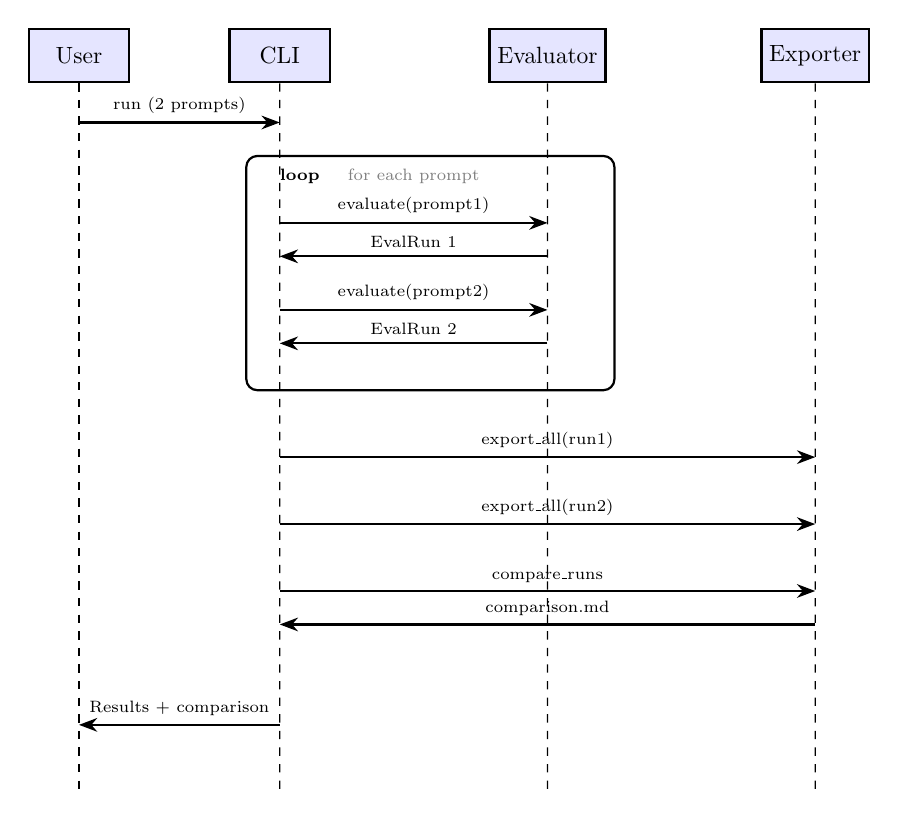
\begin{tikzpicture}[
    actor/.style={rectangle, draw=black, thick, minimum height=0.8cm, minimum width=1.5cm, fill=blue!10},
    arrow/.style={-{Stealth}, thick},
    scale=0.85, transform shape
]

% Actors
\node[actor] (user) at (0,0) {User};
\node[actor] (cli) at (3,0) {CLI};
\node[actor] (eval) at (7,0) {Evaluator};
\node[actor] (export) at (11,0) {Exporter};

% Lifelines
\draw[dashed] (user) -- (0,-11);
\draw[dashed] (cli) -- (3,-11);
\draw[dashed] (eval) -- (7,-11);
\draw[dashed] (export) -- (11,-11);

% Messages
\draw[arrow] (0,-1) -- node[above, font=\scriptsize] {run (2 prompts)} (3,-1);

% Loop box
\draw[thick, rounded corners] (2.5,-1.5) rectangle (8,-5);
\node[font=\scriptsize\bfseries] at (3.3,-1.8) {loop};
\node[font=\scriptsize, text=gray] at (5,-1.8) {for each prompt};

\draw[arrow] (3,-2.5) -- node[above, font=\scriptsize] {evaluate(prompt1)} (7,-2.5);
\draw[arrow] (7,-3) -- node[above, font=\scriptsize] {EvalRun 1} (3,-3);
\draw[arrow] (3,-3.8) -- node[above, font=\scriptsize] {evaluate(prompt2)} (7,-3.8);
\draw[arrow] (7,-4.3) -- node[above, font=\scriptsize] {EvalRun 2} (3,-4.3);

\draw[arrow] (3,-6) -- node[above, font=\scriptsize] {export\_all(run1)} (11,-6);
\draw[arrow] (3,-7) -- node[above, font=\scriptsize] {export\_all(run2)} (11,-7);
\draw[arrow] (3,-8) -- node[above, font=\scriptsize] {compare\_runs} (11,-8);
\draw[arrow] (11,-8.5) -- node[above, font=\scriptsize] {comparison.md} (3,-8.5);

\draw[arrow] (3,-10) -- node[above, font=\scriptsize] {Results + comparison} (0,-10);

\end{tikzpicture}
\caption{Multi-prompt comparison sequence}
\end{figure}

\section{Metrics Calculation Flow}

\begin{figure}[h]
\centering
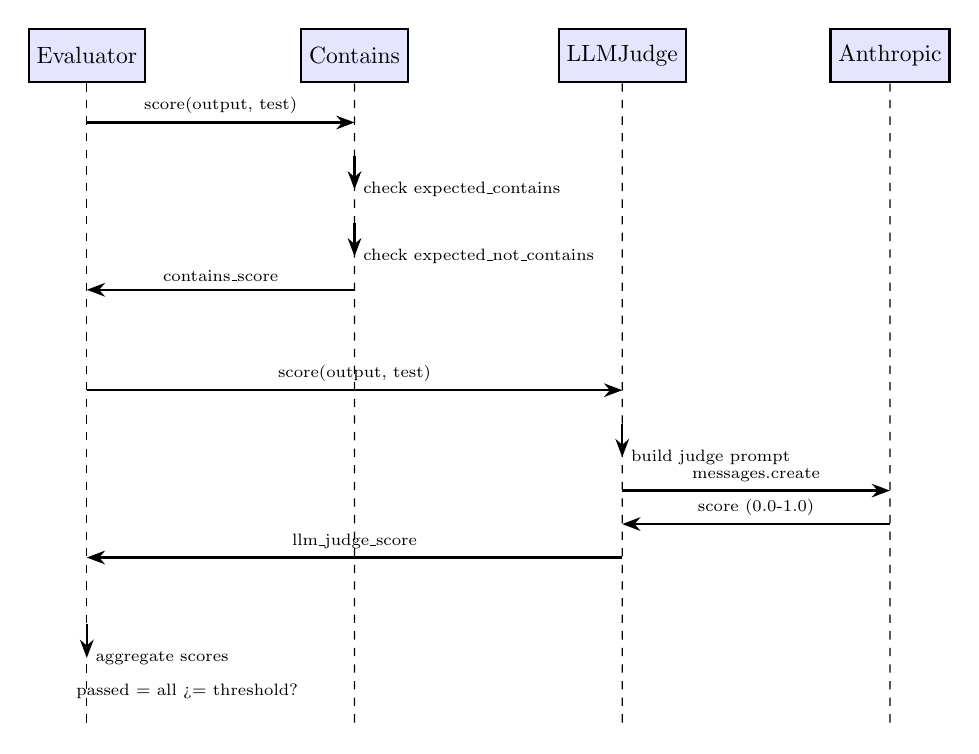
\begin{tikzpicture}[
    actor/.style={rectangle, draw=black, thick, minimum height=0.8cm, minimum width=1.5cm, fill=blue!10},
    arrow/.style={-{Stealth}, thick},
    scale=0.85, transform shape
]

% Actors
\node[actor] (eval) at (0,0) {Evaluator};
\node[actor] (contains) at (4,0) {Contains};
\node[actor] (judge) at (8,0) {LLMJudge};
\node[actor] (api) at (12,0) {Anthropic};

% Lifelines
\draw[dashed] (eval) -- (0,-10);
\draw[dashed] (contains) -- (4,-10);
\draw[dashed] (judge) -- (8,-10);
\draw[dashed] (api) -- (12,-10);

% Contains metric
\draw[arrow] (0,-1) -- node[above, font=\scriptsize] {score(output, test)} (4,-1);
\draw[arrow] (4,-1.5) -- (4,-2) node[right, font=\scriptsize] {check expected\_contains};
\draw[arrow] (4,-2.5) -- (4,-3) node[right, font=\scriptsize] {check expected\_not\_contains};
\draw[arrow] (4,-3.5) -- node[above, font=\scriptsize] {contains\_score} (0,-3.5);

% LLM Judge metric
\draw[arrow] (0,-5) -- node[above, font=\scriptsize] {score(output, test)} (8,-5);
\draw[arrow] (8,-5.5) -- (8,-6) node[right, font=\scriptsize] {build judge prompt};
\draw[arrow] (8,-6.5) -- node[above, font=\scriptsize] {messages.create} (12,-6.5);
\draw[arrow] (12,-7) -- node[above, font=\scriptsize] {score (0.0-1.0)} (8,-7);
\draw[arrow] (8,-7.5) -- node[above, font=\scriptsize] {llm\_judge\_score} (0,-7.5);

% Aggregate
\draw[arrow] (0,-8.5) -- (0,-9) node[right, font=\scriptsize] {aggregate scores};
\node[font=\scriptsize] at (1.5,-9.5) {passed = all >= threshold?};

\end{tikzpicture}
\caption{Metrics calculation sequence}
\end{figure}

% ============================================================================
% CHAPTER 10: TROUBLESHOOTING
% ============================================================================

\chapter{Troubleshooting}

\section{Common Errors}

\subsection{Error: ``ANTHROPIC\_API\_KEY not set''}

\textbf{Problem:} The API key is not configured.

\textbf{Solution:}
\begin{lstlisting}[style=bash]
# Option 1: Set environment variable
export ANTHROPIC_API_KEY=sk-ant-...

# Option 2: Create .env file
echo "ANTHROPIC_API_KEY=sk-ant-..." > .env
\end{lstlisting}

\subsection{Error: ``No prompts found in config''}

\textbf{Problem:} The configuration file doesn't specify any prompts.

\textbf{Solution:} Add a \texttt{prompts} section to your config:
\begin{lstlisting}[style=yaml]
prompts:
  - prompts/my_prompt.yaml
\end{lstlisting}

\subsection{Error: ``evaluation\_threshold is required''}

\textbf{Problem:} Missing required threshold parameter.

\textbf{Solution:} Add the threshold to your config:
\begin{lstlisting}[style=yaml]
evaluation_threshold: 0.8
\end{lstlisting}

\subsection{Error: ``File not found: prompts/xyz.yaml''}

\textbf{Problem:} The prompt file path is incorrect.

\textbf{Solutions:}
\begin{itemize}
    \item Check the file exists at the specified path
    \item Paths are relative to the config file location
    \item Use forward slashes even on Windows
\end{itemize}

\section{Performance Issues}

\subsection{Slow Evaluation Speed}

\textbf{Causes and solutions:}
\begin{enumerate}
    \item \textbf{Large number of test cases}: Run in batches or use a faster model
    \item \textbf{High max\_tokens}: Reduce if responses are shorter
    \item \textbf{No prompt caching}: Use \texttt{cached\_files} for large reference documents
\end{enumerate}

\subsection{High API Costs}

\textbf{Solutions:}
\begin{enumerate}
    \item Use prompt caching for repeated content
    \item Use a cheaper model for development:
    \begin{lstlisting}[style=bash]
prompt-eval run config.yaml -m claude-haiku-3
    \end{lstlisting}
    \item Reduce test cases during development
\end{enumerate}

\section{Unexpected Results}

\subsection{Test Failing When It Should Pass}

\textbf{Debugging steps:}
\begin{enumerate}
    \item Check the HTML report for actual output
    \item Verify \texttt{expected\_contains} strings match exactly
    \item Check for typos in expected values
    \item Review the \texttt{evaluation\_threshold} setting
\end{enumerate}

\subsection{All Tests Passing When Some Should Fail}

\textbf{Debugging steps:}
\begin{enumerate}
    \item Check if \texttt{expected\_contains} is empty (defaults to pass)
    \item Verify metrics are configured correctly
    \item Lower the \texttt{evaluation\_threshold} to be more strict
\end{enumerate}

\section{Configuration Debugging}

\textbf{Validate your configuration:}
\begin{lstlisting}[style=bash]
# Check YAML syntax
python -c "import yaml; yaml.safe_load(open('config.yaml'))"

# Run with verbose output
prompt-eval run config.yaml -v
\end{lstlisting}

\textbf{Common YAML mistakes:}
\begin{lstlisting}[style=yaml]
# Wrong: Missing quotes around special characters
expected_contains:
  - What's the answer?    # Error: apostrophe

# Correct: Quote strings with special characters
expected_contains:
  - "What's the answer?"
\end{lstlisting}

% ============================================================================
% APPENDIX
% ============================================================================

\appendix

\chapter{Reference Tables}

\section{Supported Models}

\begin{table}[h]
\centering
\begin{tabular}{@{}lp{8cm}@{}}
\toprule
\textbf{Model ID} & \textbf{Description} \\
\midrule
\texttt{claude-opus-4-5-20251101} & Most capable, best for complex tasks \\
\texttt{claude-sonnet-4-20250514} & Balanced performance and cost \\
\texttt{claude-haiku-3} & Fastest, best for simple tasks \\
\bottomrule
\end{tabular}
\caption{Supported Anthropic models}
\end{table}

\section{File Format Support}

\begin{table}[h]
\centering
\begin{tabular}{@{}llp{6cm}@{}}
\toprule
\textbf{Format} & \textbf{Extension} & \textbf{Use Case} \\
\midrule
YAML & .yaml, .yml & Configuration files \\
JSON & .json & Configuration files \\
Markdown & .md & Reference documents \\
Text & .txt & Reference documents \\
PDF & .pdf & Reference documents \\
\bottomrule
\end{tabular}
\caption{Supported file formats}
\end{table}

\section{Output Formats}

\begin{table}[h]
\centering
\begin{tabular}{@{}llp{6cm}@{}}
\toprule
\textbf{Format} & \textbf{Extension} & \textbf{Best For} \\
\midrule
JSON & .json & Programmatic processing \\
CSV & .csv & Spreadsheet analysis \\
Markdown & .md & Documentation \\
HTML & .html & Visual review \\
\bottomrule
\end{tabular}
\caption{Output formats}
\end{table}

\vfill

\begin{center}
\rule{0.5\textwidth}{0.4pt}\\[0.5cm]
\textit{Generated for Prompt Evaluation Pipeline v0.1.0}
\end{center}

\end{document}
